%package list
\documentclass{article}
\usepackage[top=3cm, bottom=3cm, outer=3cm, inner=3cm]{geometry}
\usepackage{multicol}
\usepackage{graphicx}
\usepackage{url}
%\usepackage{cite}
\usepackage{hyperref}
\usepackage{array}
%\usepackage{multicol}
\newcolumntype{x}[1]{>{\centering\arraybackslash\hspace{0pt}}p{#1}}
\usepackage{natbib}
\usepackage{pdfpages}
\usepackage{multirow}
\usepackage[normalem]{ulem}
\useunder{\uline}{\ul}{}
\usepackage{svg}
\usepackage{xcolor}
\usepackage{listings}

\lstdefinestyle{ascii-tree}{
    literate={├}{|}1 {─}{--}1 {└}{+}1 
  }
\lstset{basicstyle=\ttfamily,
  showstringspaces=false,
  commentstyle=\color{red},
  keywordstyle=\color{blue}
}
%\usepackage{booktabs}
\usepackage{caption}
\usepackage{subcaption}
\usepackage{float}
\usepackage{array}

\newcolumntype{M}[1]{>{\centering\arraybackslash}m{#1}}
\newcolumntype{N}{@{}m{0pt}@{}}


%%%%%%%%%%%%%%%%%%%%%%%%%%%%%%%%%%%%%%%%%%%%%%%%%%%%%%%%%%%%%%%%%%%%%%%%%%%%
%%%%%%%%%%%%%%%%%%%%%%%%%%%%%%%%%%%%%%%%%%%%%%%%%%%%%%%%%%%%%%%%%%%%%%%%%%%%
\newcommand{\itemEmail}{kllacma@unsa.edu.pe}
\newcommand{\itemStudent}{Kevin Andree Llacma Quispe}
\newcommand{\itemCourse}{Programacion web 2}
\newcommand{\itemCourseCode}{20200585}
\newcommand{\itemSemester}{I}
\newcommand{\itemUniversity}{Universidad Nacional de San Agustín de Arequipa}
\newcommand{\itemFaculty}{Facultad de Ingeniería de Producción y Servicios}
\newcommand{\itemDepartment}{Departamento Académico de Ingeniería de Sistemas e Informática}
\newcommand{\itemSchool}{Escuela Profesional de Ingeniería de Sistemas}
\newcommand{\itemAcademic}{2024 - A}
\newcommand{\itemInput}{-}
\newcommand{\itemOutput}{-}
\newcommand{\itemPracticeNumber}{04}
\newcommand{\itemTheme}{NodeJS + Express}
%%%%%%%%%%%%%%%%%%%%%%%%%%%%%%%%%%%%%%%%%%%%%%%%%%%%%%%%%%%%%%%%%%%%%%%%%%%%
%%%%%%%%%%%%%%%%%%%%%%%%%%%%%%%%%%%%%%%%%%%%%%%%%%%%%%%%%%%%%%%%%%%%%%%%%%%%

\usepackage[english,spanish]{babel}
\usepackage[utf8]{inputenc}
\AtBeginDocument{\selectlanguage{spanish}}
\renewcommand{\figurename}{Figura}
\renewcommand{\refname}{Referencias}
\renewcommand{\tablename}{Tabla} %esto no funciona cuando se usa babel
\AtBeginDocument{%
	\renewcommand\tablename{Tabla}
}

\usepackage{fancyhdr}
\pagestyle{fancy}
\fancyhf{}
\setlength{\headheight}{30pt}
\renewcommand{\headrulewidth}{1pt}
\renewcommand{\footrulewidth}{1pt}
\fancyhead[L]{\raisebox{-0.2\height}{
\includegraphics[width=3cm]{img/logo_episunsa.png}}}
\fancyhead[C]{\fontsize{7}{7}\selectfont	\itemUniversity \\ \itemFaculty \\ \itemDepartment \\ \itemSchool \\ \textbf{\itemCourse}}
\fancyhead[R]{\raisebox{-0.2\height}{
\includegraphics[width=1.2cm]{img/logo_abet}}}
\fancyfoot[L]{Estudiante Kevin Llacma}
\fancyfoot[C]{\itemCourse}
\fancyfoot[R]{Página \thepage}

% para el codigo fuente

\usepackage{listings}
\usepackage{color, colortbl}
\definecolor{dkgreen}{rgb}{0,0.6,0}
\definecolor{gray}{rgb}{0.5,0.5,0.5}
\definecolor{mauve}{rgb}{0.58,0,0.82}
\definecolor{codebackground}{rgb}{0.95, 0.95, 0.92}
\definecolor{tablebackground}{rgb}{0.8, 0, 0}

\lstset{frame=tb,
	language=bash,
	aboveskip=3mm,
	belowskip=3mm,
	showstringspaces=false,
	columns=flexible,
	basicstyle={\small\ttfamily},
	numbers=none,
	numberstyle=\tiny\color{gray},
	keywordstyle=\color{blue},
	commentstyle=\color{dkgreen},
	stringstyle=\color{mauve},
	breaklines=true,
	breakatwhitespace=true,
	tabsize=3,
	backgroundcolor= \color{codebackground},
}

\begin{document}
	
	\vspace*{10px}
	
	\begin{center}	
		\fontsize{17}{17} \textbf{ Informe de Laboratorio \itemPracticeNumber}
	\end{center}
	\centerline{\textbf{\Large Tema: \itemTheme}}
	%\vspace*{0.5cm}	

	\begin{flushright}
		\begin{tabular}{|M{2.5cm}|N|}
			\hline 
			\rowcolor{tablebackground}
			\color{white} \textbf{Nota}  \\
			\hline 
			     \\[30pt]
			\hline 			
		\end{tabular}
	\end{flushright}	

	\begin{table}[H]
		\begin{tabular}{|x{4.7cm}|x{4.8cm}|x{4.8cm}|}
			\hline 
			\rowcolor{tablebackground}
			\color{white} \textbf{Estudiante} & \color{white}\textbf{Escuela}  & \color{white}\textbf{Asignatura}   \\
			\hline 
			{\itemStudent \par \itemEmail} & \itemSchool & {\itemCourse \par Semestre: \itemSemester \par Código: \itemCourseCode}     \\
			\hline 			
		\end{tabular}
	\end{table}		
	
	\begin{table}[H]
		\begin{tabular}{|x{4.7cm}|x{4.8cm}|x{4.8cm}|}
			\hline 
			\rowcolor{tablebackground}
			\color{white}\textbf{Laboratorio} & \color{white}\textbf{Tema}  & \color{white}\textbf{Duración}   \\
			\hline 
			\itemPracticeNumber & \itemTheme & 04 horas   \\
			\hline 
		\end{tabular}
	\end{table}
	
	\begin{table}[H]
		\begin{tabular}{|x{4.7cm}|x{4.8cm}|x{4.8cm}|}
			\hline 
			\rowcolor{tablebackground}
			\color{white}\textbf{Semestre académico} & \color{white}\textbf{Fecha de inicio}  & \color{white}\textbf{Fecha de entrega}   \\
			\hline 
			\itemAcademic & \itemInput &  \itemOutput  \\
			\hline 
		\end{tabular}
	\end{table}
\title{Programación Web\\Laboratorio 04\\Tema: NodeJS + Express}

\maketitle


\section{Marco teórico}

\subsection{NodeJS}

\begin{itemize}
    \item Node.js es un entorno de servidor de código abierto
    \item Node.js es gratis
    \item Node.js se ejecuta en varias plataformas (Windows, Linux, Unix, Mac OS X, etc.)
    \item Node.js usa JavaScript en el servidor
    \item Sitio web : https://nodejs.org/es
\end{itemize}

\subsection{Express}

\begin{itemize}
    \item Infraestructura web rápida, minimalista y flexible para Node.js
    \item Aplicaciones web: Express es una infraestructura de aplicaciones web Node.js mínima y flexible que proporciona un conjunto sólido de características para las aplicaciones web y móviles.
    \item API: Con miles de métodos de programa de utilidad HTTP y middleware a su disposición, la creación de una API sólida es rápida y sencilla.
    \item Rendimiento: Express proporciona una delgada capa de características de aplicación web básicas, que no ocultan las características de Node.js que tanto ama y conoce.
\end{itemize}


\section{Desarollo del lab}
\subsection{Descripcion}
\textbf{Cree un teclado random para banca por internet. }
\\Para realizar la app agenda seguimos los siguientes pasos

\\.Inicializamos el proyecto y agregamos dependencias
\\.npm init -y
\\.npm install express body-parser ejs



    \begin{figure}[H]
		          \centering
		          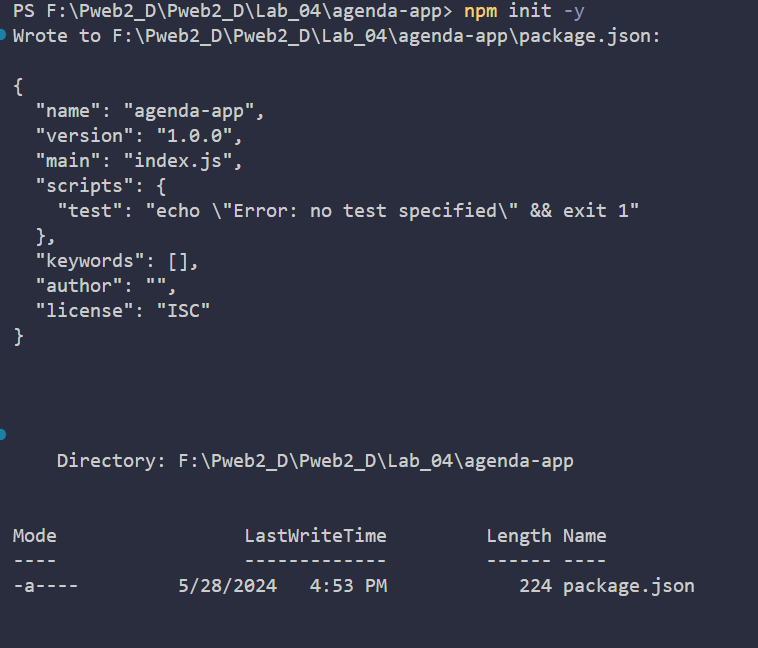
\includegraphics[width=0.8\textwidth,keepaspectratio]                       {img/dep1Agenda.png}
		             %\includesvg{img/automata.svg}
		              %\label{img:mot2}
		              %\caption{Product backlog.}
    \end{figure}
\\
    \begin{figure}[H]
		          \centering
		          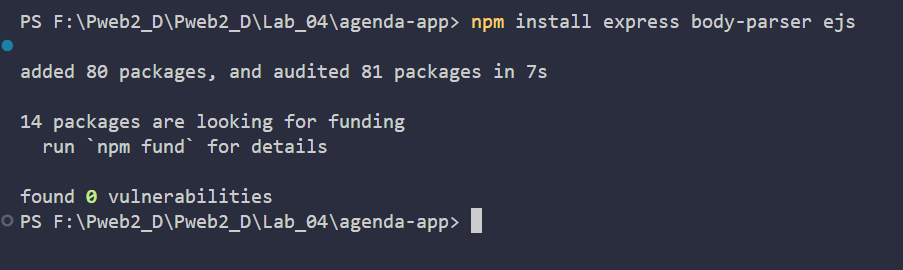
\includegraphics[width=0.8\textwidth,keepaspectratio]                       {img/dep2Agenda.png}
		             %\includesvg{img/automata.svg}
		              %\label{img:mot2}
		              %\caption{Product backlog.}
    \end{figure}

\\    

Importamos Express, body-parser para manejar los datos del formulario, y los módulos fs y path para trabajar con el sistema de archivos y las rutas.
    \begin{figure}[H]
		          \centering
		          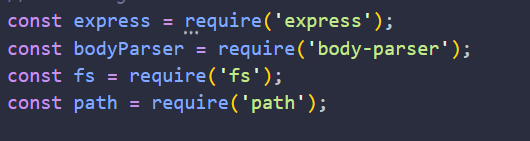
\includegraphics[width=0.8\textwidth,keepaspectratio]                       {img/modAg.png}
		             %\includesvg{img/automata.svg}
		              %\label{img:mot2}
		              %\caption{Product backlog.}
    \end{figure}
\\
Configuramos Express, habilitamos body-parser para analizar datos del formulario y configuramos EJS para plantillas.


     \begin{figure}[H]
		          \centering
		          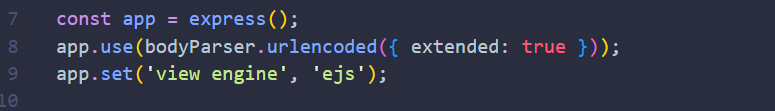
\includegraphics[width=0.8\textwidth,keepaspectratio]                       {img/confExpress.png}
		             %\includesvg{img/automata.svg}
		              %\label{img:mot2}
		              %\caption{Product backlog.}
    \end{figure}
\\
\\Definimos el directorio donde se almacenarán los eventos y nos aseguramos de que existe.
    \begin{figure}[H]
		          \centering
		          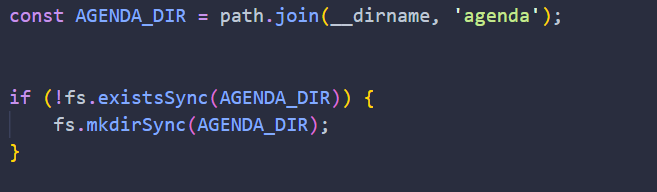
\includegraphics[width=0.8\textwidth,keepaspectratio]                       {img/confDir.png}
		             %\includesvg{img/automata.svg}
		              %\label{img:mot2}
		              %\caption{Product backlog.}
    \end{figure}
\\\textbf{getAgendaStructure():}
\\Esta función lee el directorio de la agenda y devuelve un objeto estructurado con las fechas y eventos.


    \begin{figure}[H]
		          \centering
		          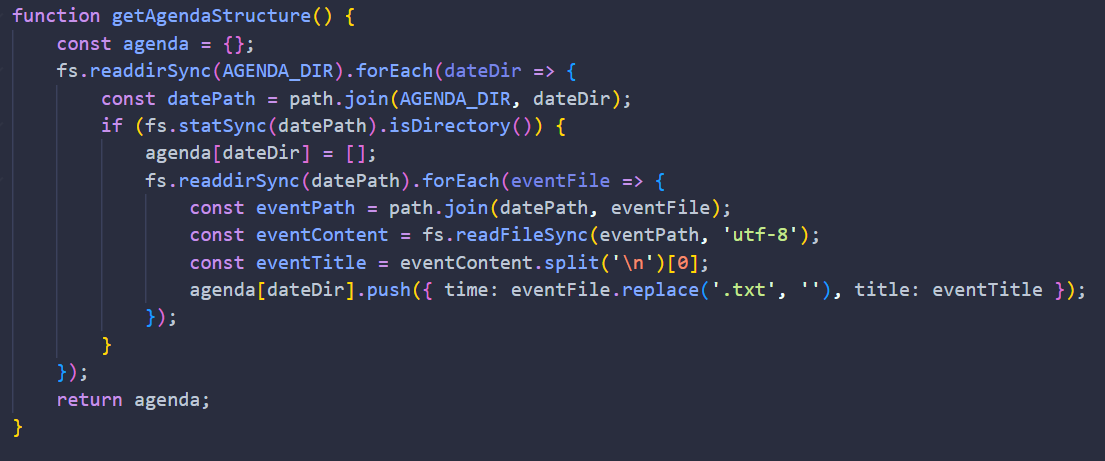
\includegraphics[width=0.8\textwidth,keepaspectratio]                       {img/strucAg.png}
		             %\includesvg{img/automata.svg}
		              %\label{img:mot2}
		              %\caption{Product backlog.}
    \end{figure}
\\Utilizamos fs.readdirSync para leer el contenido del directorio AGENDADIR. Este método devuelve una lista de nombres de archivos y directorios dentro de AGENDADIR. Iteramos sobre cada elemento utilizando forEach.

    \begin{figure}[H]
		          \centering
		          
\includegraphics[width=0.8\textwidth,keepaspectratio]                       {img/dirAg.png}
		             %\includesvg{img/automata.svg}
		              %\label{img:mot2}
		              %\caption{Product backlog.}
    \end{figure}

\\Para cada elemento en AGENDADIR, construimos la ruta completa utilizando path.join. Esto nos da la ruta completa del subdirectorio que corresponde a una fecha específica.

     \begin{figure}[H]
		          \centering
		          
\includegraphics[width=0.8\textwidth,keepaspectratio]                       {img/rutaFec.png}
		             %\includesvg{img/automata.svg}
		              %\label{img:mot2}
		              %\caption{Product backlog.}
    \end{figure}

\\Utilizamos fs.statSync para obtener información sobre datePath. Si datePath es un directorio (isDirectory()), continuamos con el procesamiento.

     \begin{figure}[H]
		          \centering
		          
\includegraphics[width=0.8\textwidth,keepaspectratio]                       {img/ifAg.png}
		             %\includesvg{img/automata.svg}
		              %\label{img:mot2}
		              %\caption{Product backlog.}
    \end{figure}
Luego
\begin{itemize}
    \item Se verifica si datePath es un directorio.
    \item Se inicializa un arreglo vacío para almacenar los eventos de la fecha.
    \item Se leen todos los archivos dentro del directorio de la fecha.
    \item Para cada archivo de evento, se construye su ruta completa.
    \item Se lee el contenido del archivo de evento.
    \item Se extrae el título del evento (la primera línea del contenido del archivo).
    \item Se agrega un objeto que contiene la hora y el título del evento al arreglo correspondiente a la fecha.
\end{itemize}

    \begin{figure}[H]
		          \centering
		          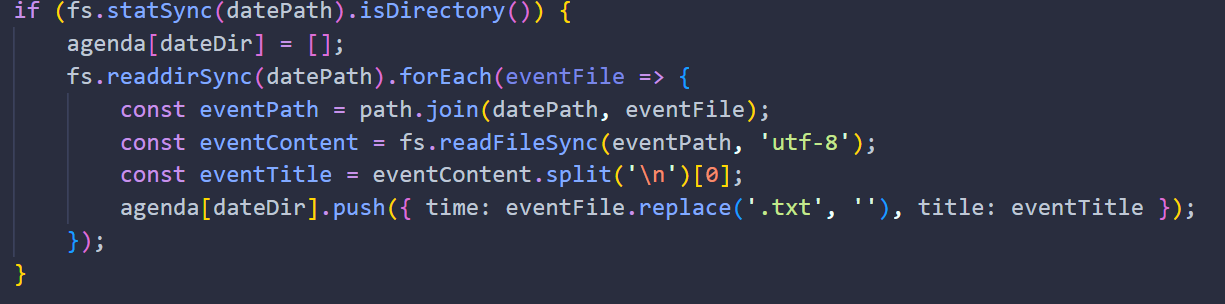
\includegraphics[width=0.8\textwidth,keepaspectratio]                       {img/ifCon.png}
		             %\includesvg{img/automata.svg}
		              %\label{img:mot2}
		              %\caption{Product backlog.}
    \end{figure}
    
\\Obtiene la estructura de la agenda y la pasa a la vista index.ejs.

    \begin{figure}[H]
		          \centering
		          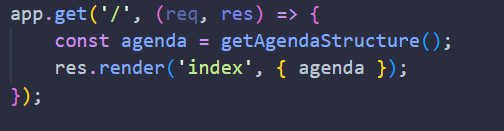
\includegraphics[width=0.8\textwidth,keepaspectratio]                       {img/home.png}
		             %\includesvg{img/automata.svg}
		              %\label{img:mot2}
		              %\caption{Product backlog.}
    \end{figure}

\\
Recibe datos del formulario, crea un nuevo evento y redirige a la página principal si el evento no existe.

    \begin{figure}[H]
		          \centering
		          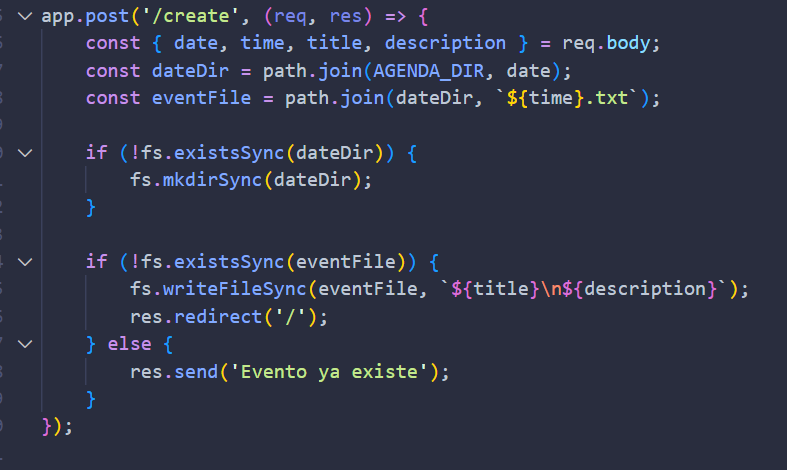
\includegraphics[width=0.8\textwidth,keepaspectratio]                       {img/crearEv.png}
		             %\includesvg{img/automata.svg}
		              %\label{img:mot2}
		              %\caption{Product backlog.}
    \end{figure}    
\\
Obtiene los detalles del evento para mostrarlos en un formulario de edición y luego actualiza el archivo con los cambios.
     \begin{figure}[H]
		          \centering
		          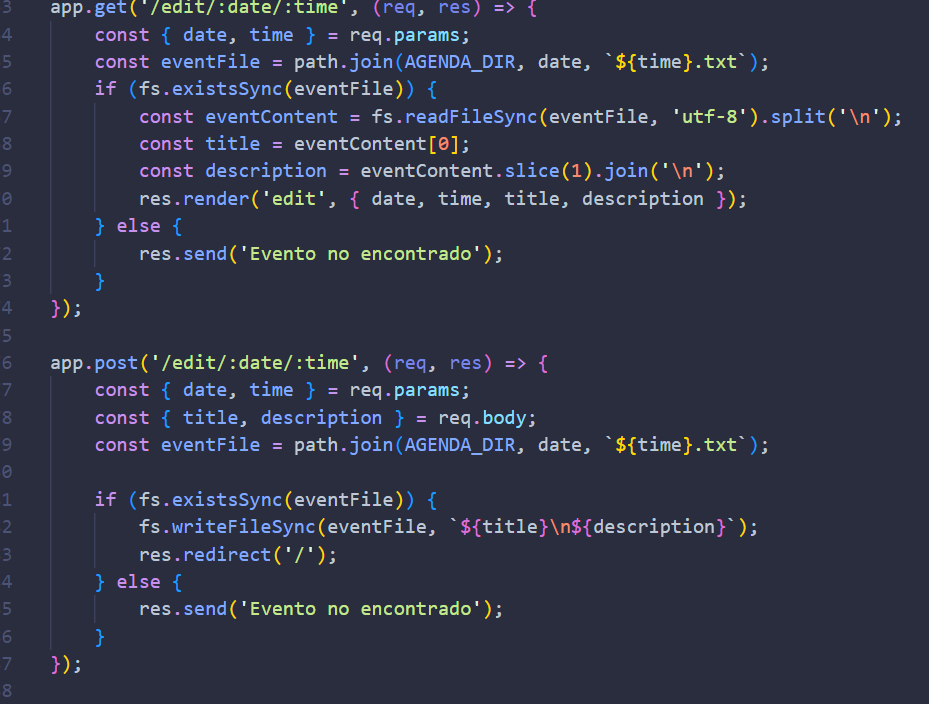
\includegraphics[width=0.8\textwidth,keepaspectratio]                       {img/editarEv.png}
		             %\includesvg{img/automata.svg}
		              %\label{img:mot2}
		              %\caption{Product backlog.}
    \end{figure}    

\\Elimina el archivo del evento y redirige a la página principal.

     \begin{figure}[H]
		          \centering
		          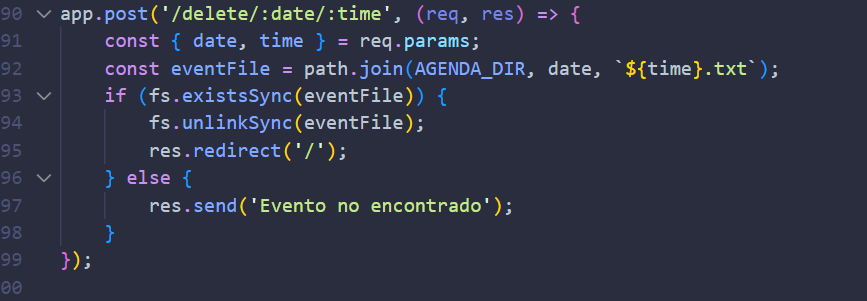
\includegraphics[width=0.8\textwidth,keepaspectratio]                       {img/eliEv.png}
		             %\includesvg{img/automata.svg}
		              %\label{img:mot2}
		              %\caption{Product backlog.}
    \end{figure}  
\\
\\Inicia el servidor en el puerto 3000 y muestra un mensaje en la consola.


 \begin{figure}[H]
		          \centering
		          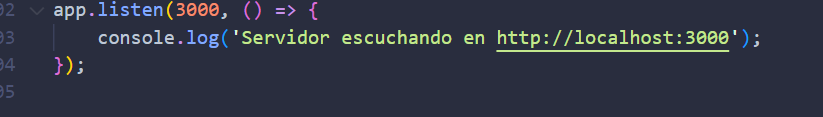
\includegraphics[width=0.8\textwidth,keepaspectratio]                       {img/iniSer.png}
		             %\includesvg{img/automata.svg}
		              %\label{img:mot2}
		              %\caption{Product backlog.}
    \end{figure}  
\\

\\Prueba de la agenda:

\begin{figure}[H]
		          \centering
		          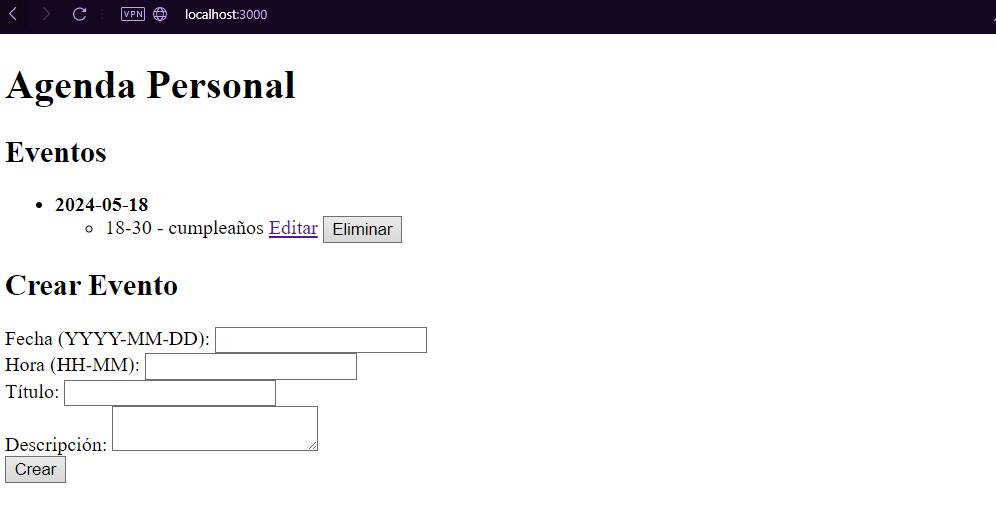
\includegraphics[width=0.8\textwidth,keepaspectratio]                       {img/pruebaAg.png}
		             %\includesvg{img/automata.svg}
		              %\label{img:mot2}
		              %\caption{Product backlog.}
    \end{figure}  
\\

\begin{figure}[H]
		          \centering
		          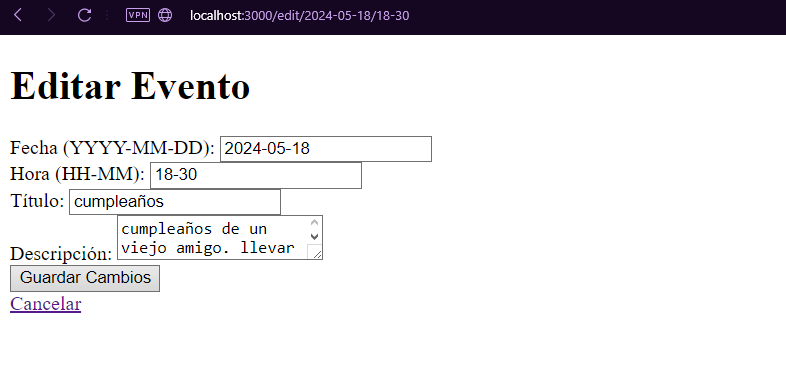
\includegraphics[width=0.8\textwidth,keepaspectratio]                       {img/prueba2Ag.png}
		             %\includesvg{img/automata.svg}
		              %\label{img:mot2}
		              %\caption{Product backlog.}
    \end{figure} 
Se uso docker file para correr la aplicacion:

    \begin{figure}[H]
		          \centering
		          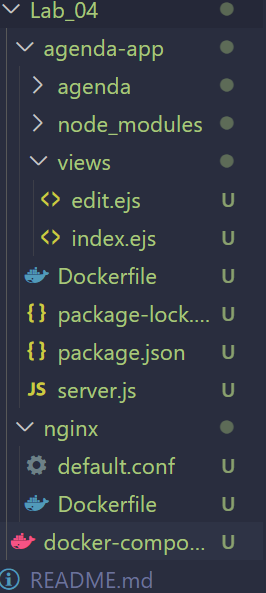
\includegraphics[width=0.5\textwidth,keepaspectratio]                       {img/dockerAg.png}
		             %\includesvg{img/automata.svg}
		              %\label{img:mot2}
		              %\caption{Product backlog.}
    \end{figure} 

\begin{itemize}
    \item Define la imagen base node:14.
    \item Establece el directorio de trabajo en /usr/src/app.
    \item Copia los archivos package.json y package-lock.json y ejecuta npm install para instalar las dependencias.
    \item Copia el resto del código de la aplicación.
    \item Expone el puerto 3000.
    \item Define el comando para iniciar la aplicación.
\end{itemize}

 \begin{figure}[H]
		          \centering
		          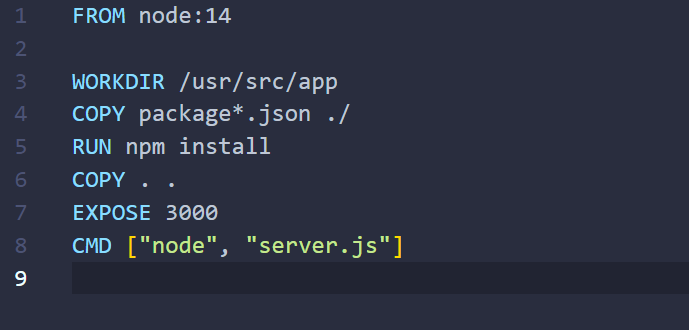
\includegraphics[width=0.5\textwidth,keepaspectratio]                       {img/dockerNode.png}
		             %\includesvg{img/automata.svg}
		              %\label{img:mot2}
		              %\caption{Product backlog.}
    \end{figure} 

\begin{itemize}
    \item Define que Nginx escuche en el puerto 80.
    \item Configura la ubicación raíz / para pasar las solicitudes a la aplicación NodeJS en http://node:3000.
    \item Configura la ubicación /static para servir archivos estáticos directamente desde el directorio public de la aplicación.
\end{itemize}
     \begin{figure}[H]
		          \centering
		          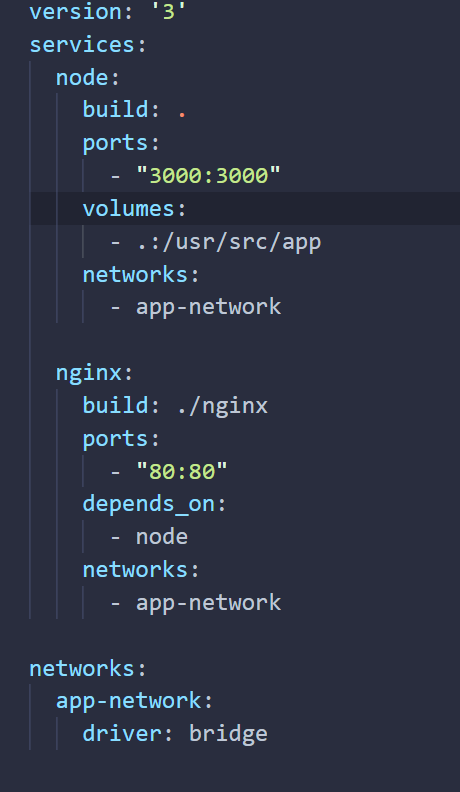
\includegraphics[width=0.5\textwidth,keepaspectratio]                       {img/dockercom.png}
		             %\includesvg{img/automata.svg}
		              %\label{img:mot2}
		              %\caption{Product backlog.}
    \end{figure} 

\end{document}